\section{Performance Analysis}\label{sec:performance analysis}
To test the performance of my code I designed two scripts which automated my
analysis. In the file \textit{test\_population.sh} there is code for running 20
runs of my code with population sizes from 10 to 20. The code uses different
random variables so we can get a proper average. The other settings was
"crossover=0.5", "mutation=0.025", "elite=5" which means that it has a one point
crossover, approximately one mutation per gene and the 5 best\footnote{If this is
possible, for some population sizes this means that only the best are used for
mating} are used for mating no matter what. I then use another script
\textit{average.py} to take the average over all which is then plotted using
\textit{plot\_population\_average.gnuplot}. In figure
\ref{fig:population-average} you can see the result of all the runs\footnote{In
	many of the plots there is no standard deviation or average plotted,
	this is done because including them would mean so much clutter that it
would be impossible to interpret anything useful from the plots}.

\begin{figure}[h!]
	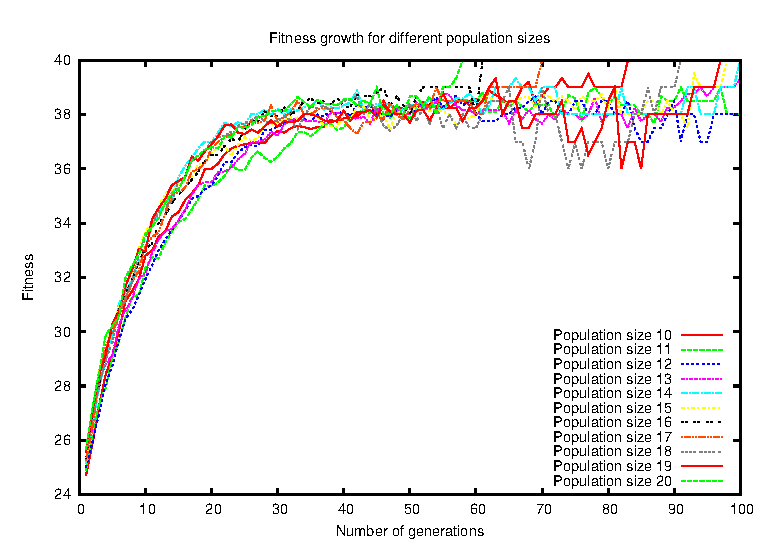
\includegraphics{../graphs/fitness_population_average.eps}
	\caption{Average fitness growth for the best individual for different populations}
	\label{fig:population-average}
\end{figure}

As can be seen from the plot there is no clear winner, several reaches the max
fitness within 100 generations and some don't. This is also dependant on the
random seed selected. For this reason I will continue forward with a population
size of 15, because I'm quite sure that it should always make it. On previous
runs I have also seen it do quite a bit better so I'm quite confident that 15 is
a good size to chose.

When testing for crossover and mutation rate the task was a bit more difficult
to plot concise. For this reason I made a another script,
\textit{test\_crossover.sh}, which can test a lot of different mutation and
crossover rates. The problem is plotting this. I haven't found a pretty way of
showing it, so below I include two out of seven plots\footnote{There should be
no problem recreating the results and looking at them}, one containing the best
results and one showing that it did not improve much. For the plots I have run
20 times with different seeds for each of the 20 times, but the same seed for
different crossovers and mutation rates. I used a population size of 15 as said
above and elitism of 5 to keep it consistent with the test ran above.

\begin{figure}[h!]
	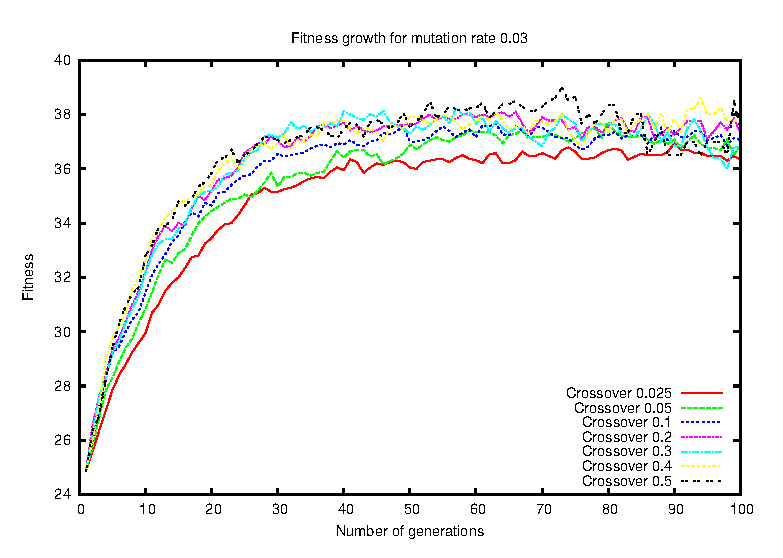
\includegraphics{../graphs/fitness_crossover_mute_003_average.eps}
	\caption{Average fitness for the best individual with a mutation rate of 0.03 and all the
	different crossover rates tested for}
	\label{fig:cross 0.03}
\end{figure}

\begin{figure}[h!]
	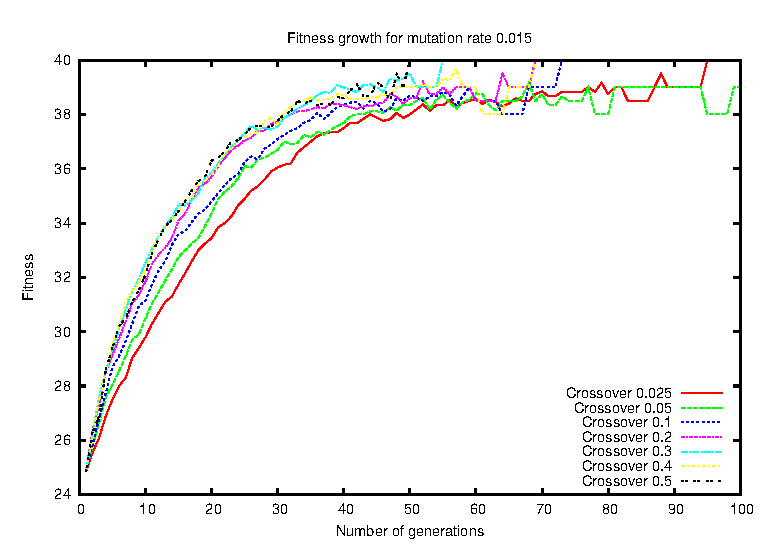
\includegraphics{../graphs/fitness_crossover_mute_0015_average.eps}
	\caption{Average fitness of the best individual with a mutation rate of 0.015 and all the
	different crossover rates tested for}
	\label{fig:cross 0.015}
\end{figure}

In figure \ref{fig:cross 0.015} we can see that with a crossover rate of 0.5 and
a mutation rate of 0.015 we can solve the \textit{One-Max problem} in around 50
generations\footnote{This was the lowest of all the seven runs, but random seed
	will affect this, so this might not be exactly the same for other
runs, but I think that average of 20 runs should yield good results}

\subsection{Selection Mechanism}\label{sec:selection mechanism}
When testing for the best selection mechanism I again started by making a new
script for automated testing, \textit{test\_selection.sh}. This files run
through all of the different selection mechanisms that I have implemented,
namely \textit{Fitness Proportionate}, \textit{Sigma Scaling}, \textit{Rank
Selection} and \textit{Tournament Selection}. The result can be seen below in
figure \ref{fig:selection}.

\begin{figure}[h!]
	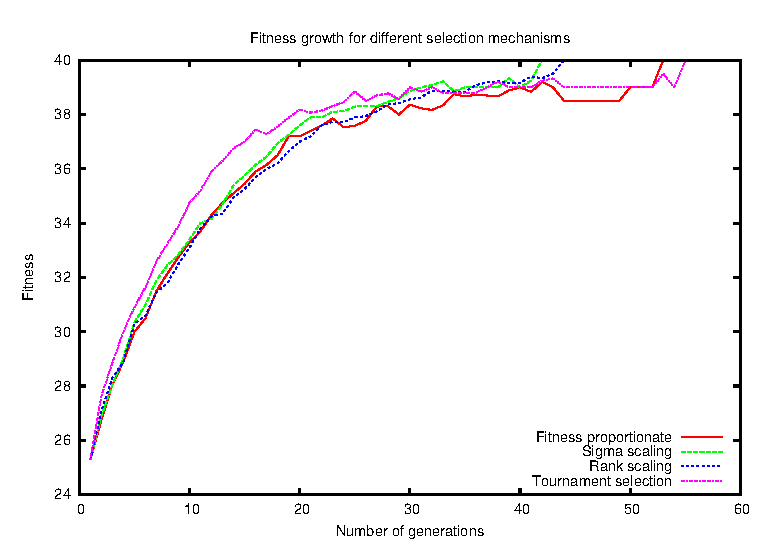
\includegraphics{../graphs/fitness_selection_average.eps}
	\caption{Average fitness of the best individuals with different
	selection mechanisms}
	\label{fig:selection}
\end{figure}

From this we can see that both Sigma scaling and Rank selection do a very good
job and
improve quite a lot on Fitness Proportionate. Tournament selection does lag a
bit behind, but this also have some parameters that would need tuning for better
results. For this task I decided to try and tweak them some, but there is room for improvement.

\subsection{Random Target}\label{sec:random target}
For this task I ran a new script which generated 40bit long random strings and
ran four different tests, again with 20 different runs. In figure
\ref{fig:random target} we can see the results. If we compare this with the
results obtained in figure \ref{fig:selection} we can see that there really is
not that much difference between them. Even tough it is a bit quicker in figure
\ref{fig:selection} that can easily be attributed to random and as such I
conclude that trying to evolve a random target is no different from an all one
target. This makes sense since in many ways an all one target is no different
from a randomly chosen different bit string. As an example say we have a random
target which must have a "101" somewhere inside and a random phenotype in the
population which contains "111" converting between those two are no different from the
one max problem going the other way, and as such is no different.

\begin{figure}[h!]
	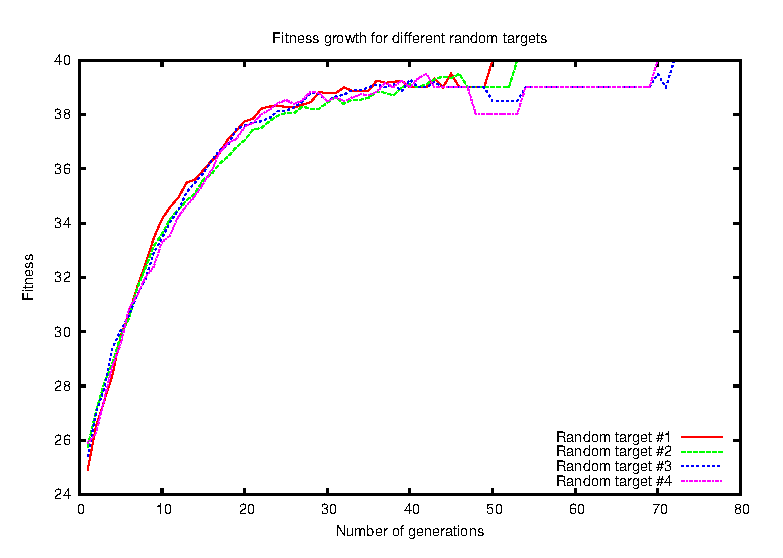
\includegraphics{../graphs/fitness_target_average.eps}
	\caption{Average fitness of the best individual with four different
	randomly generated target bit strings}
	\label{fig:random target}
\end{figure}
